\chapter{Trabalhos Correlatos}\label{trabalhos-correlatos}

Com o intuito de contextualizar e ter uma melhor visão de onde posicionar o projeto dentro do campo de pesquisa escolhido, foi realizada uma seleção de trabalhos correlatos, cujos principais critérios de aceitação incluíram a abordagem de temas como: monitoramento de fauna, desenvolvimento sustentável, gestão ambiental e ciência cidadã. Garantindo assim, relevância e alinhamento do projeto com as necessidades e avanços da área.

O ponto de partida para as pesquisas foi o \citeonline{sibbr2024}. A plataforma online, pertencente ao sistema gov.br \cite{govbr2024}, que integra dados e informações sobre a biodiversidade e os ecossistemas de diversas fontes, os tornando acessíveis e livres para usos diversos. Nele, também é possível ter acesso ao sistema Ciência Cidadã, que consiste em uma colaboração entre a comunidade e cientistas na coleta de dados para pesquisa científica. 

A partir do levantamento bibliográfico, pesquisas na plataforma Play Store \cite{playstore2024}, presente nos dispositivos Android \cite{android2024}, foram realizadas baseadas em alguns projetos e palavras-chave pré-selecionadas. As principais palavras-chave usadas para realizar as buscas foram: animais costeiros, coleta de dados, monitoramento ambiental, ciência cidadã.

Nesta seção, serão apresentadas três aplicações separadas no levantamento documental que  demonstraram possuir características e funcionalidades que podem auxiliar na definição e desenvolvimento deste sistema. Estas aplicações possuem algumas características em comum, porém cada uma delas também traz características únicas que serão importantes balizadoras nas tomadas de decisão deste projeto.

% ---
\section{SISS-Geo}\label{siss-geo}
% --- 

O Sistema de Informação em Saúde Silvestre (SISS-Geo) da FIOCRUZ é desenvolvido pela Plataforma Institucional Biodiversidade e Saúde Silvestre, com apoio do Laboratório Nacional de Computação Científica. É gratuito, disponível em \textit{smartphones} e na \textit{web}, para o monitoramento da saúde dos animais silvestres em ambientes naturais, rurais e urbanos. Apoia a investigação da ocorrência de agentes causadores de doenças, como agentes infecciosos, que podem acometer pessoas e animais. Como instrumento de ciência cidadã torna possível, a partir de registros realizados por cidadãos comuns, profissionais de saúde, meio ambiente, pesquisadores e especialistas em vida silvestre, agir para a prevenção e controle de zoonoses e a conservação da biodiversidade brasileira \cite{chame2015sissgeo}.

\begin{figure}[htb]
  \centering
  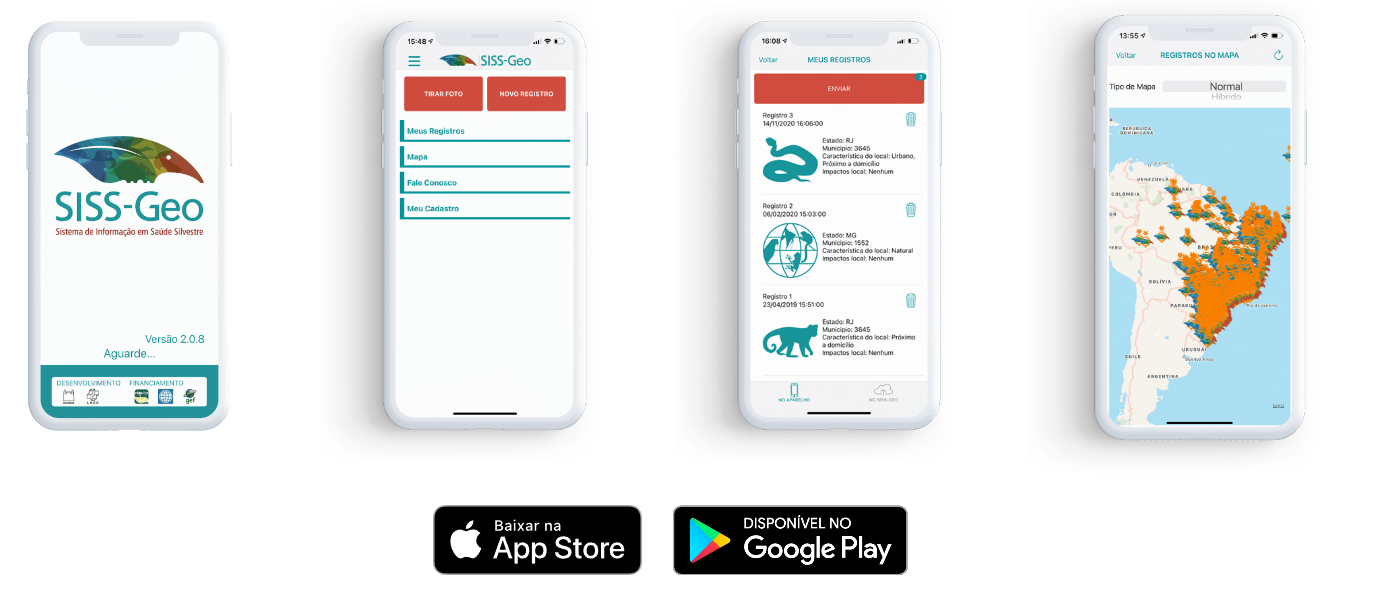
\includegraphics[width=1\textwidth]{imagens/sisGeoApp.png}
  \caption{Interface do sistema SISS-Geo.}
  \legend{Fonte: \citeonline{plataforma2024sissgeo}.}
  \label{fig:sisgeoApp}
\end{figure}

A aplicação \textit{mobile} foi lançada em 2014 e está disponível tanto para IOS quanto para Android (Figura~\ref{fig:sisgeoApp}) e possui mais de 10.000 downloads, com avaliação média de 4,7/5 baseada em 116 avaliações de usuários. Foram registrados, até 26 de março de 2024, 33 mil registros e quase 13 mil usuários colaboradores.

O sistema é bem consolidado e amplamente utilizado no Brasil, possuindo uma ótima aceitação entre especialistas e cidadãos em diversas regiões do país. Apesar de possuir opções para identificação de dados da fauna costeira, estes se mostram limitados quando comparados com os demais biomas. Ao alterar a escala de análise, é possível perceber, com um recorte mais detalhado do cordão litorâneo, que este não é o principal foco da aplicação e, atualmente, ela possui uma participação muito maior nas regiões continentais (Figura~\ref{fig:sisgeoMap}).

\begin{figure}[htb]
  \centering
  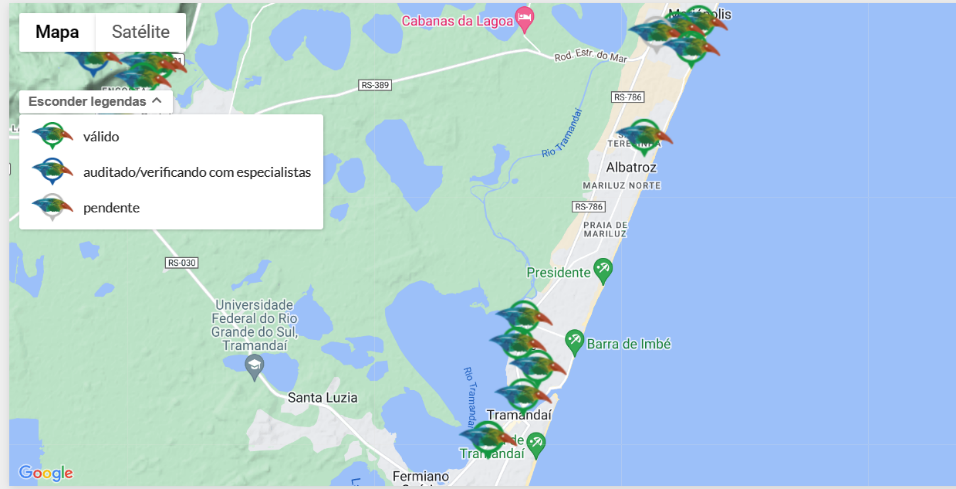
\includegraphics[width=1\textwidth]{imagens/sisGeoMapa.png}
  \caption{Recorte da região costeira do litoral norte do Rio Grande do Sul.}
  \legend{Fonte: \citeonline{plataforma2024sissgeo}.}
  \label{fig:sisgeoMap}
\end{figure}

Principais pontos fortes: funcionalidade \textit{offline}, iniciativa ambiental de grande contribuição, aplicação leve, ideia colaborativa de preservação, georreferenciamento de dados com boa visualização.

Entre as principais reclamações dos usuários estão: sistema pouco intuitivo, poucas opções de animais pré-cadastrados, interface confusa com formulário por vezes muito técnico.

% ---
\section{Sistema Urubu}\label{urubu}
% --- 

O Sistema Urubu é uma iniciativa do Centro Brasileiro de Ecologia de Estradas da UFLA, sob a coordenação do professor Alex Bager. Criado em 2014, o aplicativo de ciência cidadã é a maior rede para conservação da biodiversidade brasileira, destinada à coleta e gestão de informações de fauna selvagem ao longo de rodovias e ferrovias no Brasil. 

A aplicação permite que voluntários enviem registros de animais atropelados e infraestruturas viárias por meio de aplicativo móvel, enquanto especialistas validam e caracterizam esses registros para torná-los confiáveis. Os dados coletados são centralizados em um banco de dados e disponibilizados em um Sistema de Informações Geográficas, facilitando a visualização e análise pelos usuários. O Sistema Urubu também oferece ferramentas como o Urubu \textit{web}, para gestão e validação dos dados, e o Urubu Map, para visualização geográfica dos registros \cite{castro2019sistema}. Ao longo de seus anos de existência, o sistema reuniu mais de 25 mil usuários e 150 mil registros de animais atropelados em todo o território brasileiro, demonstrando seu impacto e relevância na conservação da biodiversidade.

\begin{figure}[htb]
  \centering
  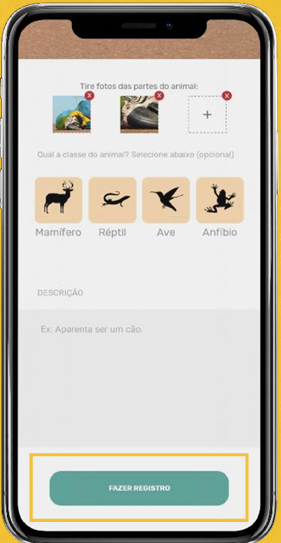
\includegraphics[width=0.33\textwidth]{imagens/app1.png}
  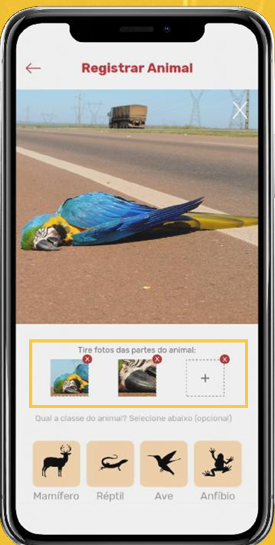
\includegraphics[width=0.323\textwidth]{imagens/app3.png}
  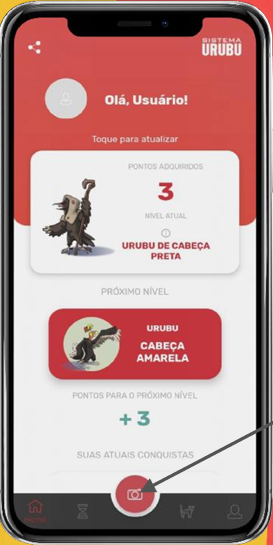
\includegraphics[width=0.32\textwidth]{imagens/app2.png}
  \caption{Interface do Sistema Urubu.}
  \legend{Fonte: Capturas de tela do sistema urubu disponíveis no manual de uso do aplicativo.}
  \label{fig:urubuApp}
\end{figure}

O Sistema Urubu apresenta uma interface amigável e um fluxo de obtenção e envio de dados de registros intuitivo (Figura~\ref{fig:urubuApp}.a e ~\ref{fig:urubuApp}.b), além de um fluxo gamificado com progressão recompensada para os usuários que contribuem com o projeto (Figura~\ref{fig:urubuApp}.c).

O fluxo de funcionamento da aplicação se inicia com a morte de algum animal em uma rodovia ou ferrovia, quando esse animal é encontrado por usuário a entrada de registro pode ser realizada via \textit{mobile}, \textit{web} ou por importação via planilha de Excel. Os dados de cada registro são então passados por uma análise de profissionais que decidirão se serão inseridos nos dados finais.

Apesar de ter alcançado importantes números de aceitação e uso entre 2014 e 2023, atualmente o sistema se encontra desativado e indisponível para download em todas as plataformas e seu site se encontra fora do ar.

Em contato com o coordenador do projeto Alex Brag por e-mail, foi informado de que o Sistema Urubu foi desativado devido a falta de recursos. Segundo seu relato, além dos custos para manter a aplicação no ar com investimentos contínuos, os aplicativos de ciência cidadã requerem muita comunicação e relacionamento com os participantes, o que torna a estrutura mais complexa e custosa.

% ---
\section{SIMBA}\label{simba}
% --- 

O Sistema de Monitoramento da Biota Aquática (SIMBA), é um sistema \textit{web} de gerenciamento de dados criado pelo Laboratório de Oceanografia Biológica da UNIVALI com a finalidade de armazenar dados coletados por instituições executoras dos projetos de monitoramentos de praias. O desenvolvimento do SIMBA se iniciou para auxiliar nos fluxos de dados entre os atores sociais envolvidos nos Projetos de Monitoramento de Praias (PMPs) e fazer com que os dados obtidos sejam disponibilizados e divulgados para a população.

Os PMPs são desenvolvidos para o atendimento de condicionantes de licenciamento ambiental federal, conduzido pelo IBAMA, de atividades de exploração e produção de petróleo e gás natural de bacias \textit{offshore} sob atuação da Petrobras. Estes projetos tem o objetivo de avaliar as possíveis interferências na área de abrangência dos projetos, analisando tanto tetrápodes marinhos (aves, tartarugas e mamíferos) por meio do monitoramento das praias, atendimento veterinário aos animais debilitados e da coleta de dados de animais mortos, quanto resíduos sólidos encontrados \cite{petrobras_simba_2024}.

Atualmente os projetos estão presentes nas bacias de Santos, Campos, Espírito Santo, Sergipe-Alagoas e Potiguar.

\begin{figure}[htb]
  \centering
  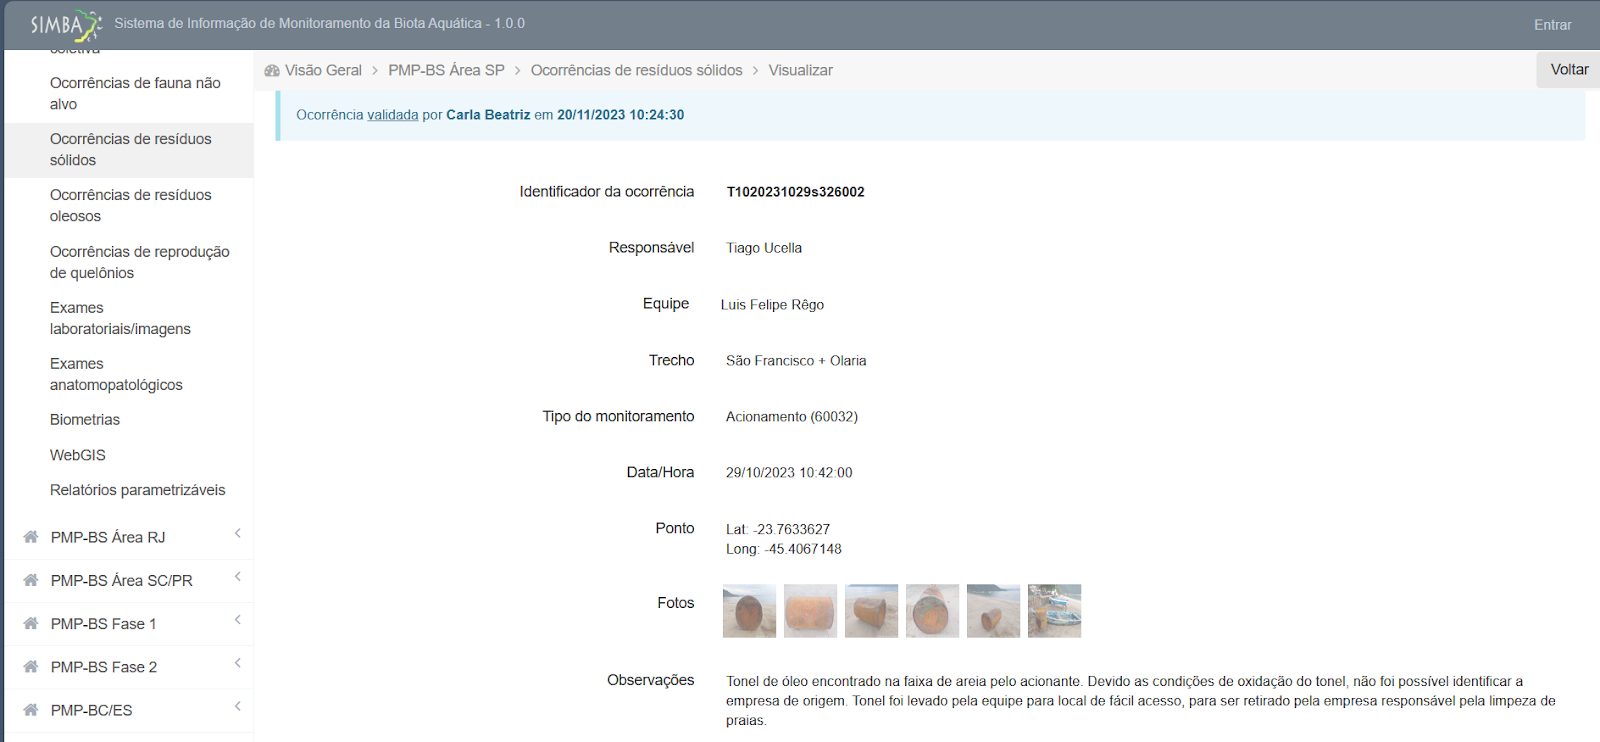
\includegraphics[width=1\textwidth]{imagens/simbaRegistro.png}
  \caption{Captura de tela de uma página \textit{web} de registro de visualização de ocorrências cadastradas no SIMBA.}
  \legend{Fonte: \cite{petrobras_simba_2024}.}
  \label{fig:simbaRegistro}
\end{figure}

O SIMBA conta com funcionalidades de cadastro de ocorrências de fauna, resíduos sólidos (Figura~\ref{fig:simbaRegistro}), exames, jornadas de campo com os caminhamentos realizados. Os pontos de ocorrência de cada cadastro são georreferenciados, assim como as jornadas de monitoramento, gerando mapas para melhor visualização e análise dos dados (Figura~\ref{fig:simbaMonitoramento}).

\begin{figure}[htb]
  \centering
  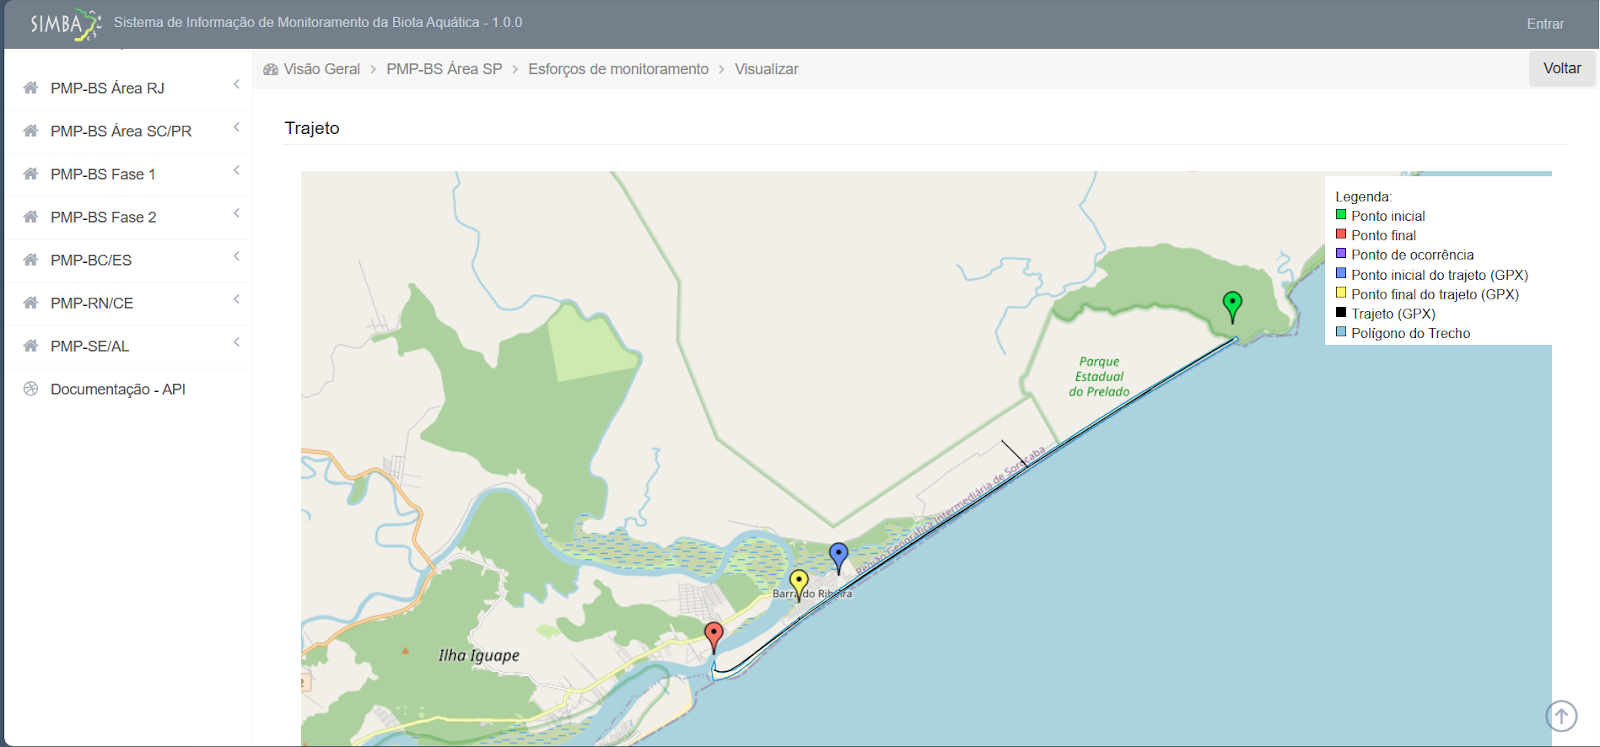
\includegraphics[width=1\textwidth]{imagens/simbaTrajetoria.png}
  \caption{Captura de tela de um mapa georreferenciado gerado a partir dos dados de jornada de monitoramento cadastrado no SIMBA.}
  \legend{Fonte: \cite{petrobras_simba_2024}.}
  \label{fig:simbaMonitoramento}
\end{figure}

O sistema possui uma área de acesso liberada ao público onde é possível visualizar dados já levantados e validados e uma área de acesso restrito liberada para pesquisadores. Possui uma interface mais limpa e direta, atendendo a um estilo de aplicação profissional apenas com o conteúdo necessário (Figura~\ref{fig:simbaPaginaCadastro}). Os dados são bem organizados e acessíveis para quem estiver interessado em acompanhar os estudos e evidências coletadas. Porém, para leigos essa interface pode, inicialmente, trazer um pouco de estranheza devido ao visual menos apelativo e aos termos mais científicos apresentados.

\begin{figure}[htb]
  \centering
  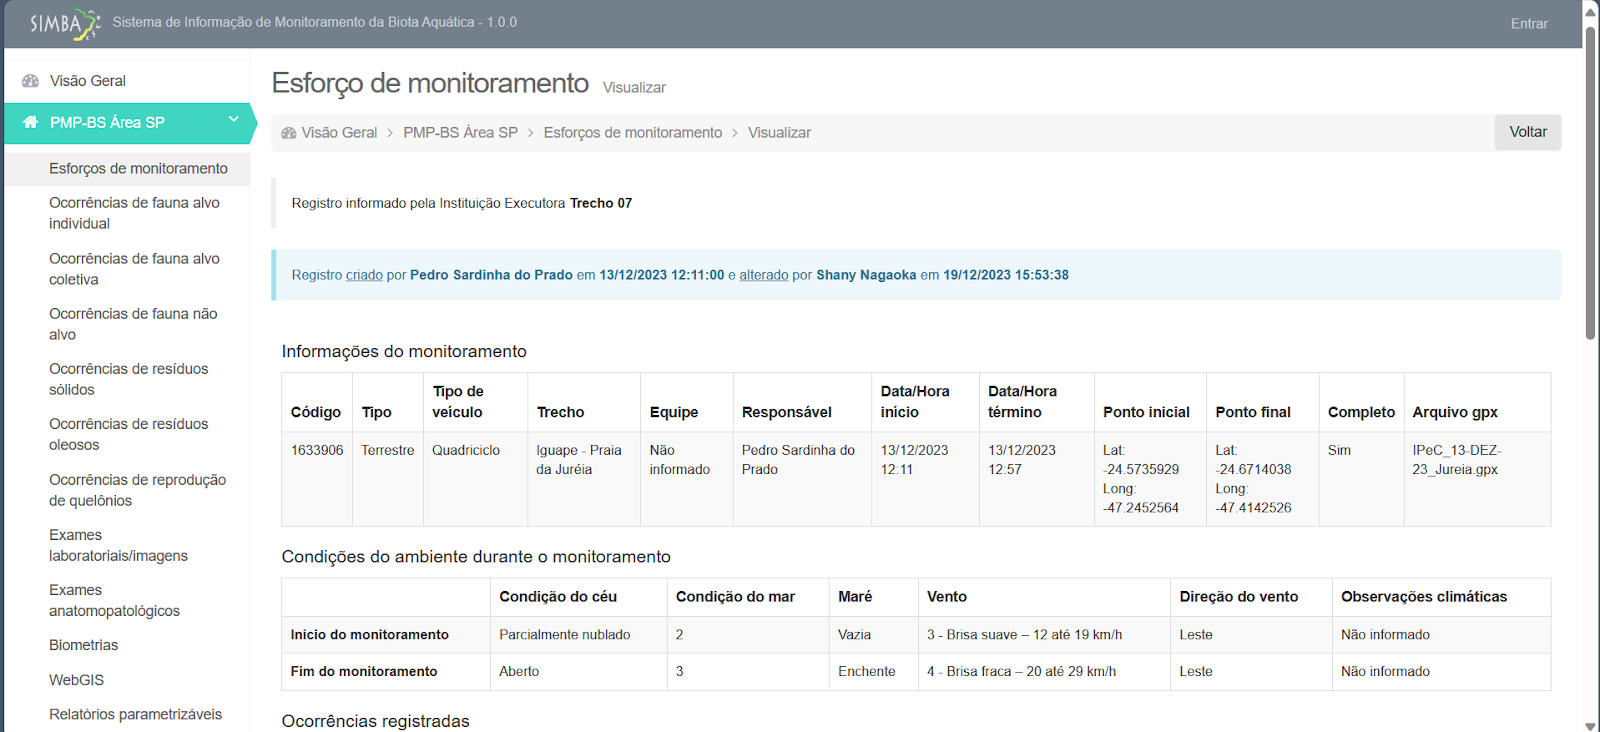
\includegraphics[width=1\textwidth]{imagens/simbaMonitoramento.png}
  \caption{Captura de tela da página \textit{web} de monitoramento cadastrada no SIMBA.}
  \legend{Fonte: \cite{petrobras_simba_2024}.}
  \label{fig:simbaPaginaCadastro}
\end{figure}

A geração de mapas georreferenciados e a possibilidade de uso \textit{offline} são aspectos importantes a serem destacados, pois permitem uma melhor análise e acompanhamento gráfico dos dados coletados e possibilitam que estes dados sejam obtidos até mesmo em locais mais isolados sem conexão com a internet. Outra função interessante é a liberação de dados para o público geral que se mostrar interessado em acompanhar os resultados e andamentos dos estudos nas praias onde os PMPs estão sendo realizados.

\section{Análise Comparativa e Direcionamentos do Projeto}

Com a análise dos principais trabalhos correlatos existentes, foi possível levantar os principais pontos de sucesso e alguns aspectos que precisam de melhorias, os quais influenciam diretamente na capacidade de sistemas similares alcançarem seus objetivos e obterem a aceitação do público-alvo.

A receptividade do Sistema Urubu e do SISS-Geo indicou um interesse significativo da população em participar de projetos de ciência cidadã, evidenciado pelos números expressivos de \textit{downloads} e registros de dados apresentados anteriormente.

Cada um dos três sistemas possui suas peculiaridades e objetivos distintos: enquanto o SISS-Geo está mais voltado ao monitoramento da saúde de animais silvestres e à investigação de agentes causadores de doenças, o Sistema Urubu foca principalmente no monitoramento de animais atropelados em rodovias e ferrovias. Por sua vez, o SIMBA busca fornecer visibilidade ao monitoramento costeiro realizado em regiões de exploração e produção de petróleo.

Sendo assim, a partir da análise prévia, foi possível constatar que existe uma oportunidade de posicionamento para o sistema proposto neste projeto, que se enquadra como uma plataforma com interface amigável e intuitiva, visando otimizar o processo de coleta, classificação e gestão de dados da fauna costeira. O sistema poderá se apoiar em pontos fortes identificados nos sistemas correlatos, como a funcionalidade offline do SISS-Geo, a interface amigável do Sistema Urubu e a organização dos dados do SIMBA.

O sistema proposto buscará oferecer uma experiência de usuário agradável e descomplicada para o registro de observações da fauna costeira, com opções abrangentes de espécies para classificação e ferramentas de visualização de dados claras e acessíveis. Ao adotar uma abordagem centrada no usuário e priorizar a simplicidade e eficiência, pretende-se ampliar o engajamento da comunidade na coleta de dados científicos e contribuir significativamente para o monitoramento e conservação da biodiversidade costeira.
